\section{Controller}

The Figure \ref{fig:desiredpoints} shows the points that will be targeting the controller to reach from the initial position (marked in red). 

\begin{figure}[h!] 
    \centering
    \begin{subfigure}[b]{0.45\linewidth}
        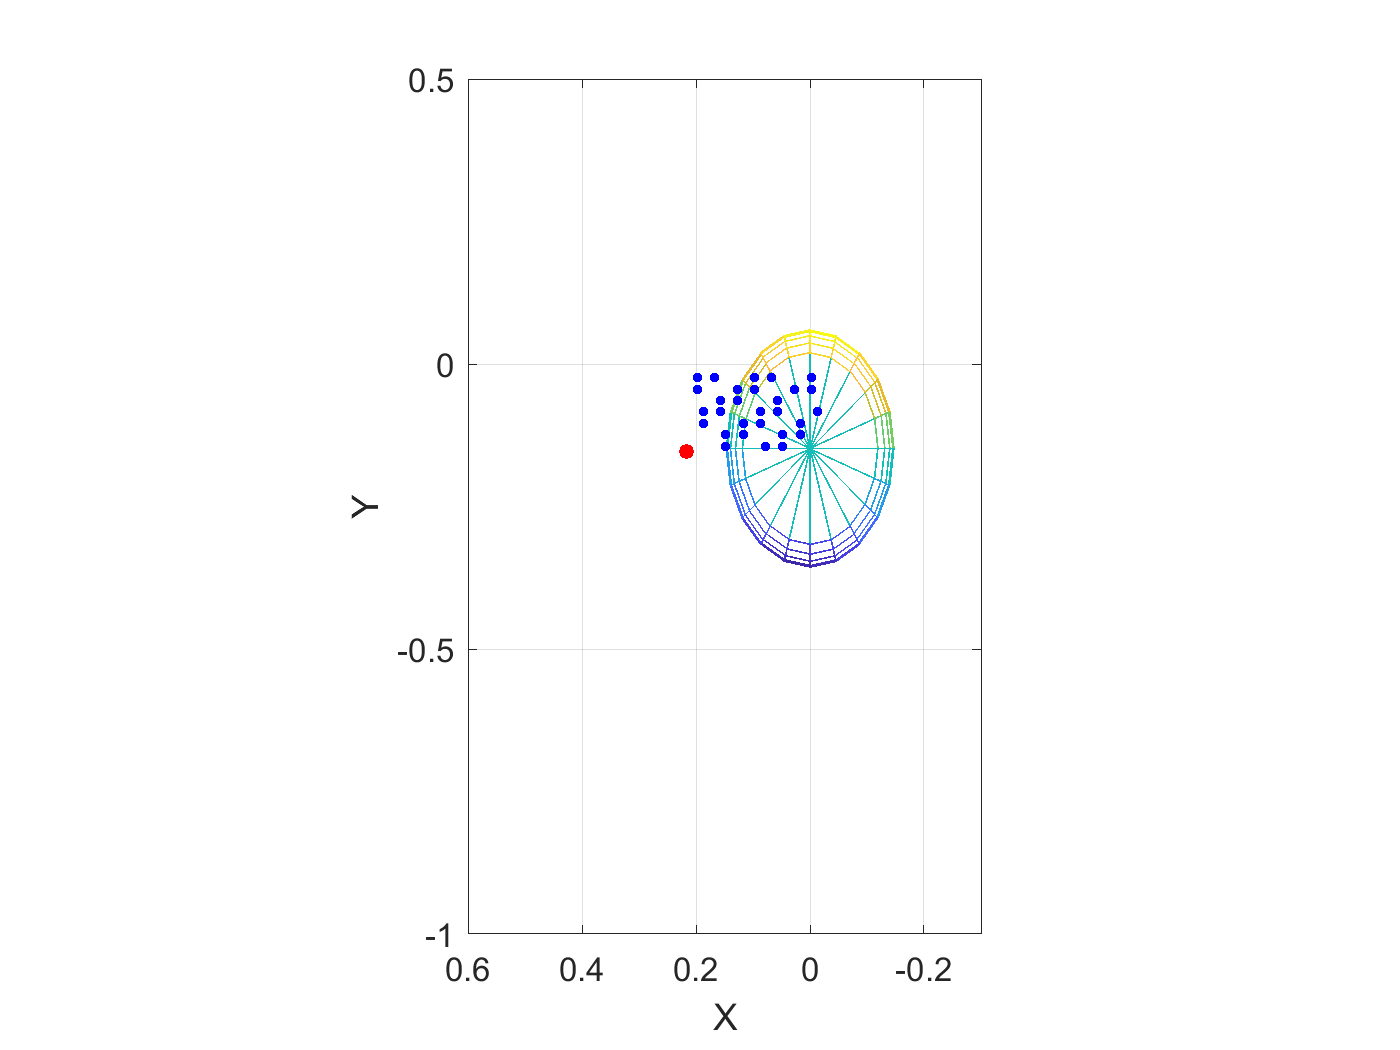
\includegraphics[width=0.7\textwidth]{Pictures/Results/Controller/DesiredPointsFV.png}
    \end{subfigure}
    \hfill
    %\vspace{1cm} % Adjust the space between the figures as needed
    \begin{subfigure}[b]{0.45\linewidth}            
        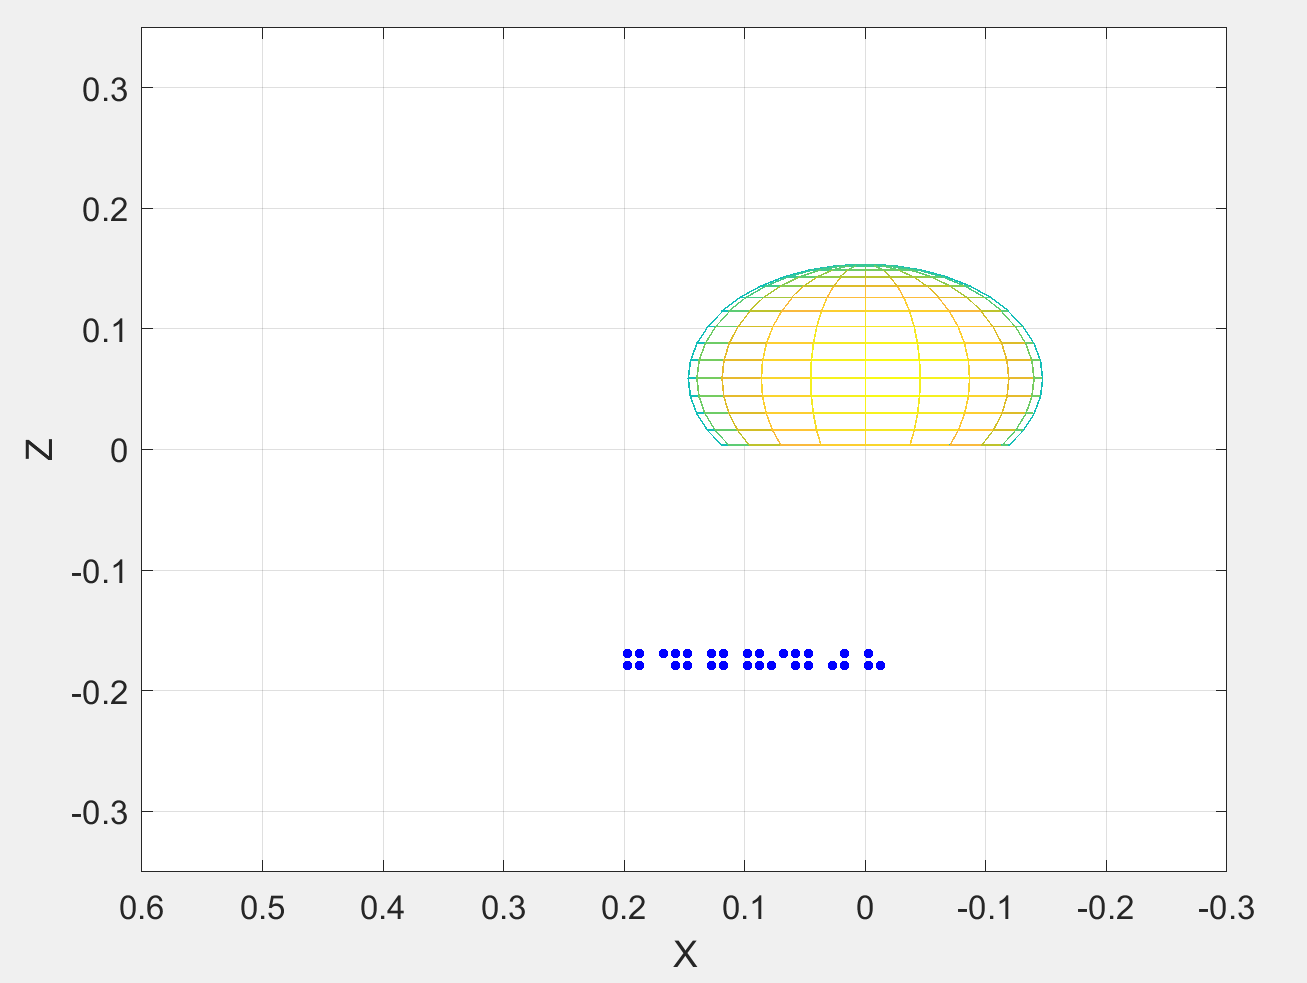
\includegraphics[width=\textwidth]{Pictures/Results/Controller/DesiredPointsSV.png}
    \end{subfigure}
    \caption{Desired Targets for Reaching in Rehabilitation Task (Front View, Side View)}
    \label{fig:desiredpoints}
\end{figure}

\subsection{Static Control}
\begin{figure}[h!]
\centering
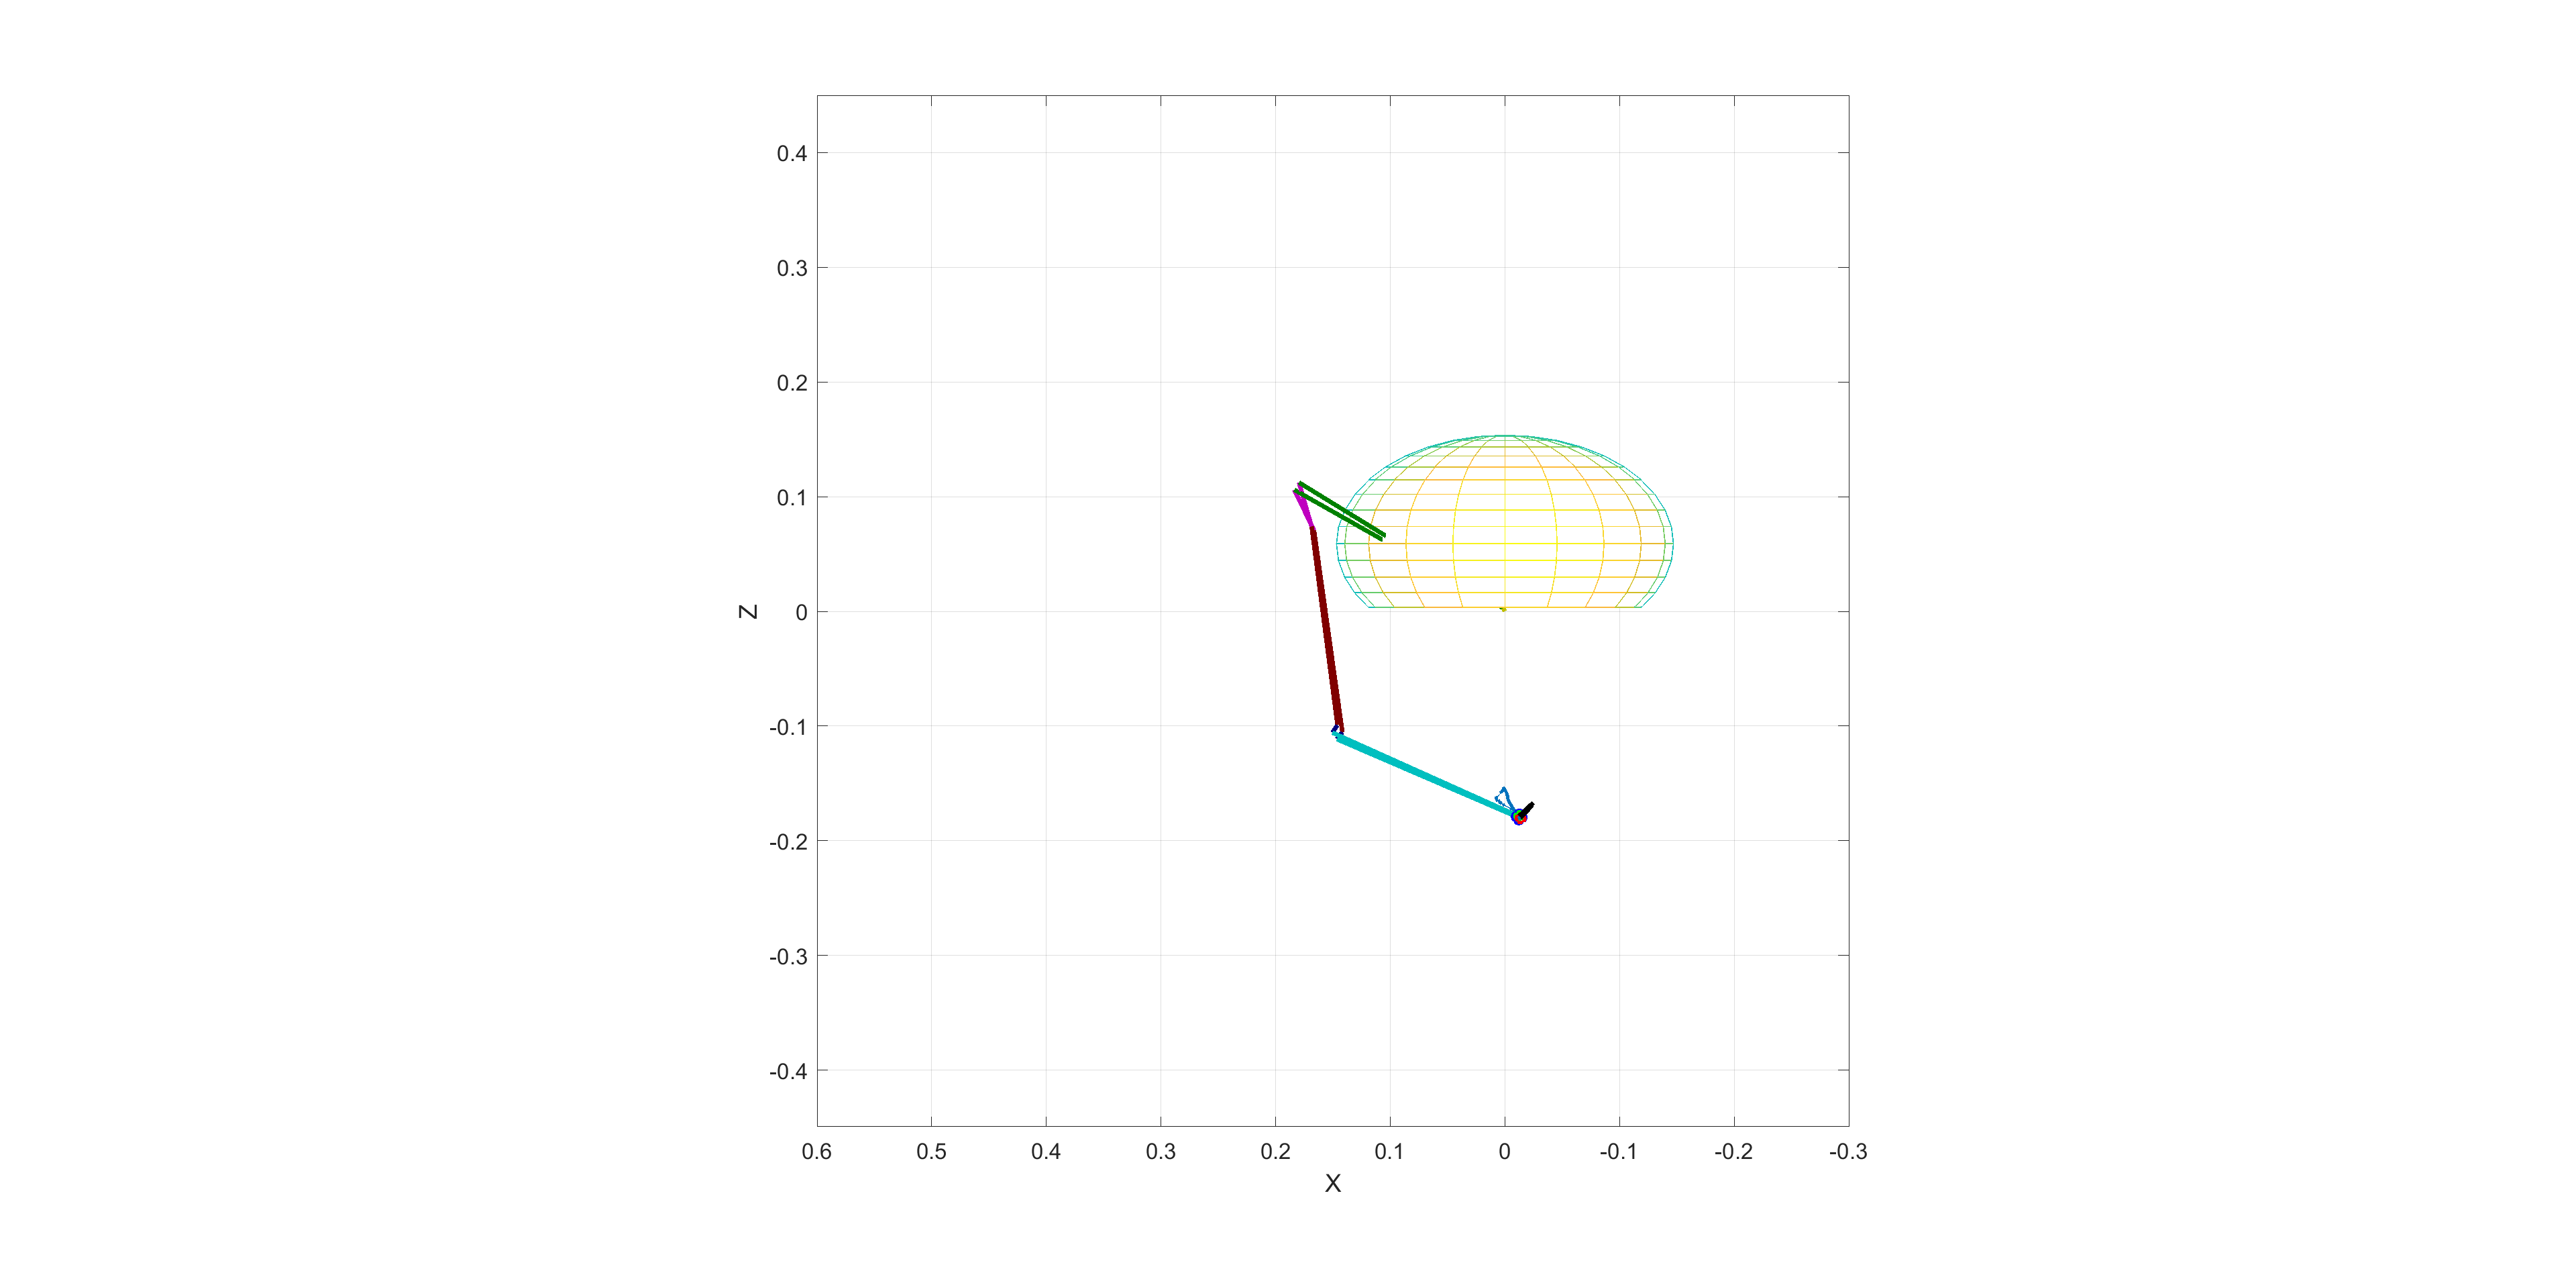
\includegraphics[width=1\textwidth]{Pictures/Controller/StaticControl_WP.png} 
\caption{Static Control Example Wrist Position Configuration} % Optional caption
\label{fig:SCWP} % Optional label for referencing
\end{figure}

\begin{figure}[h!]
\centering
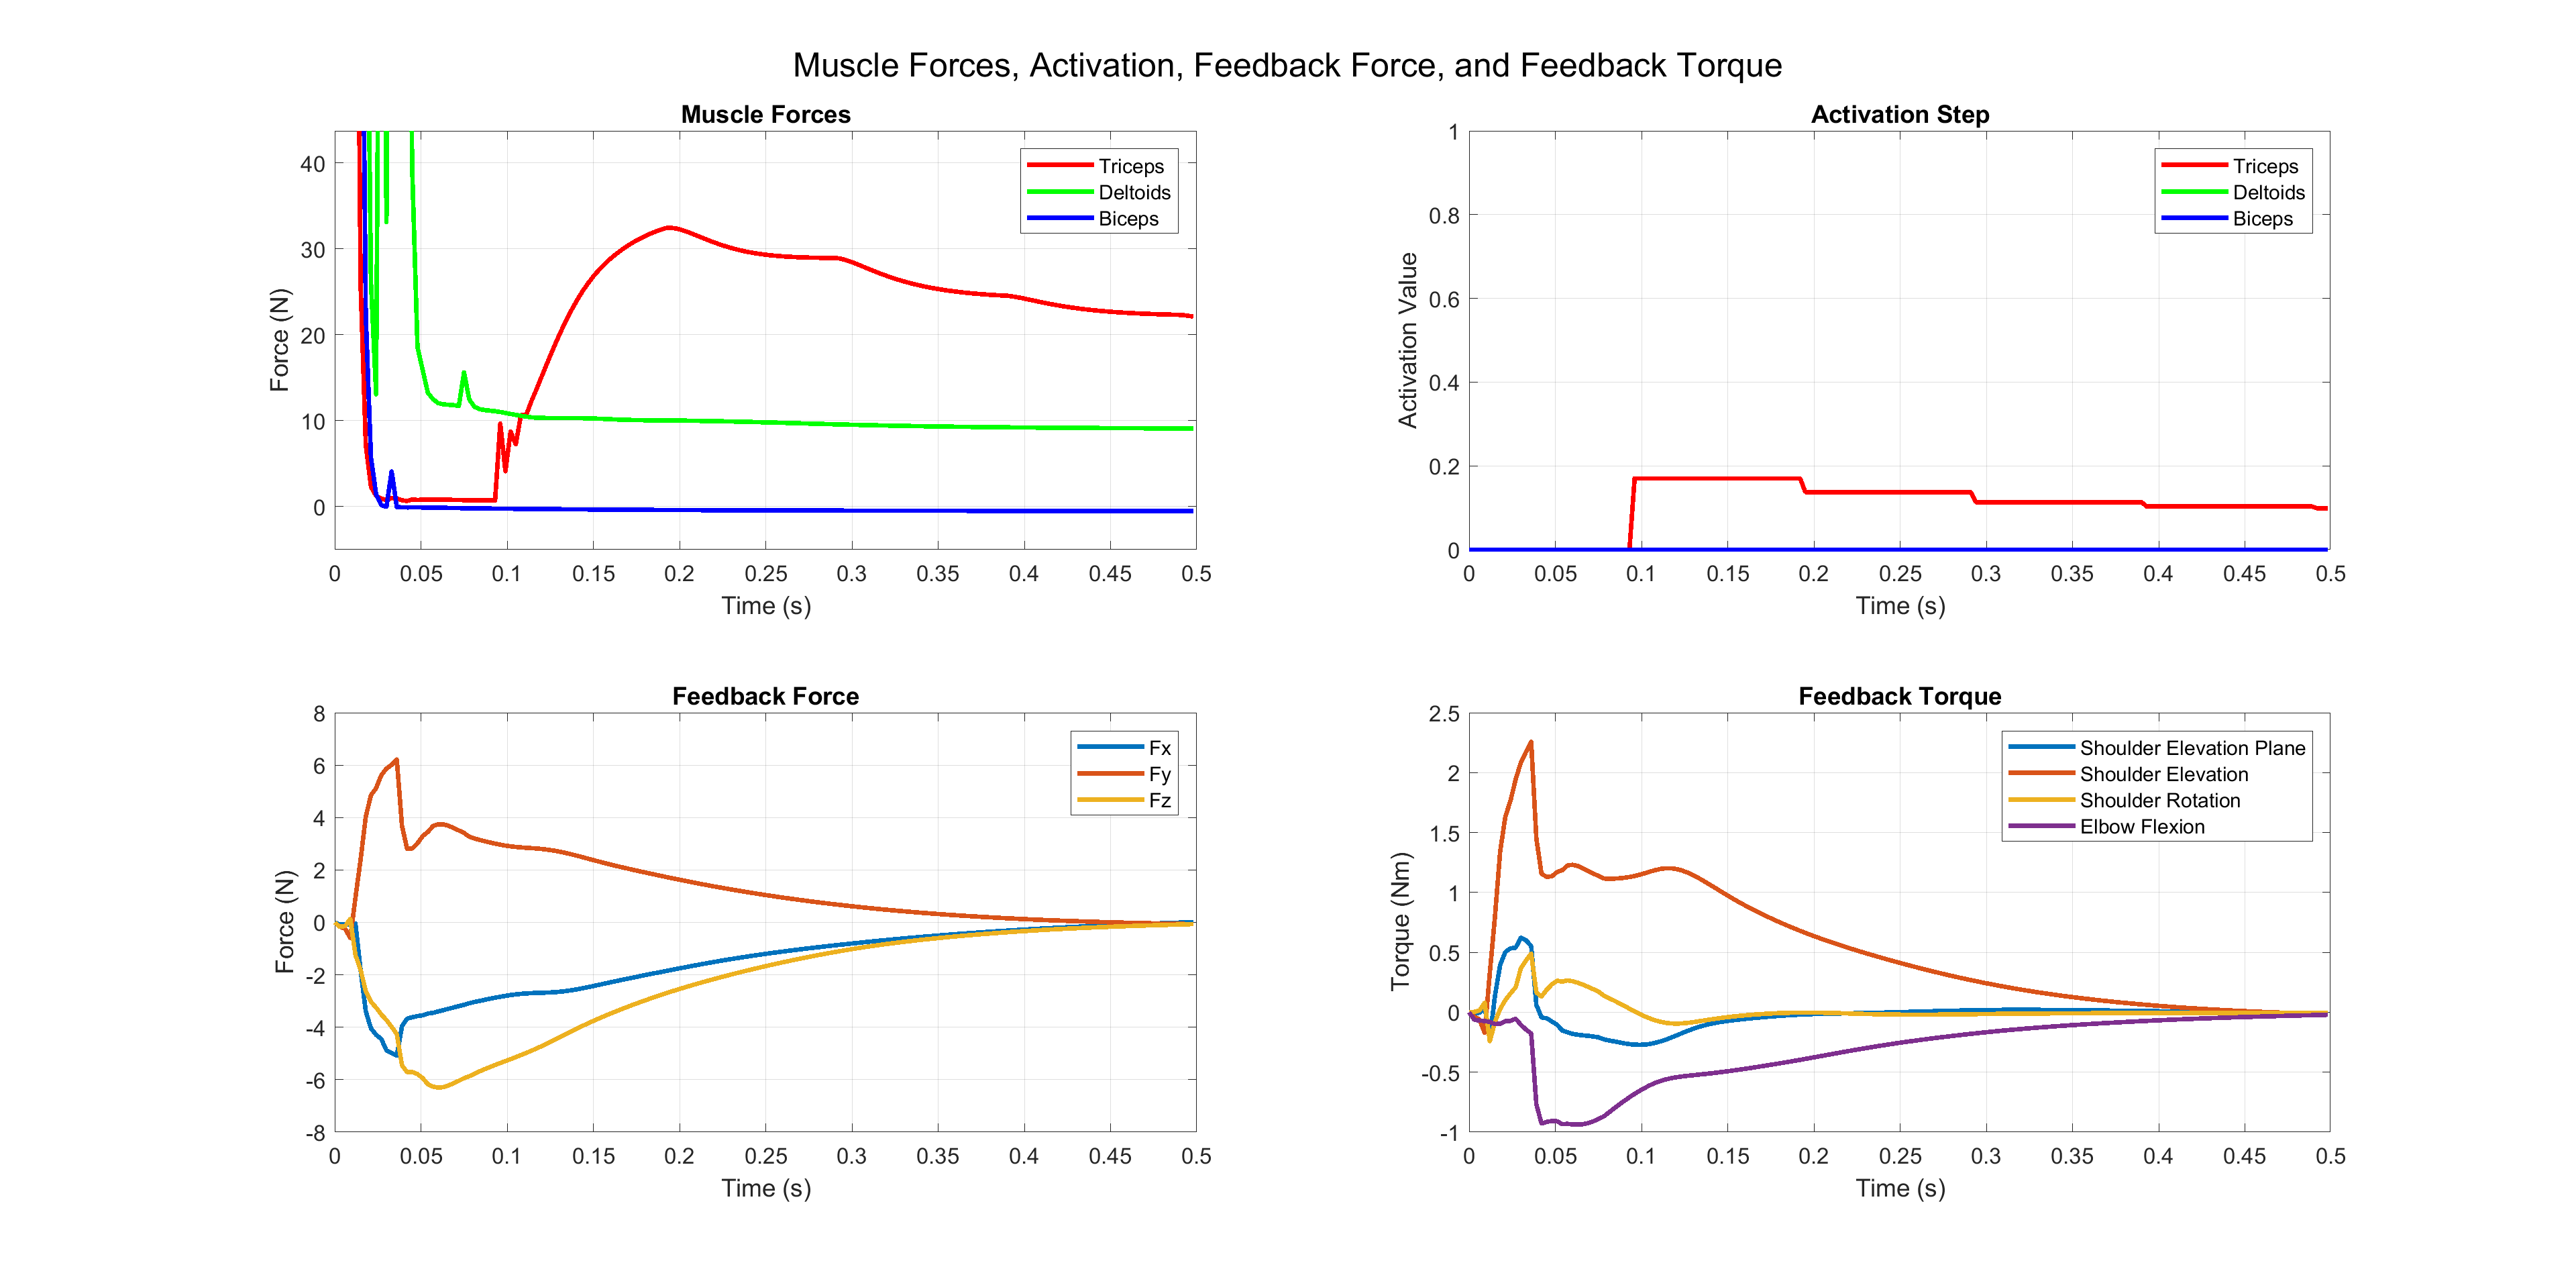
\includegraphics[width=1\textwidth]{Pictures/Controller/StaticControl.png} 
\caption{Static Control Example Muscle Forces, Activation Step, Feedback Force and Feedback Torque } % Optional caption
\label{fig:SC} % Optional label for referencing
\end{figure}
\newpage
\begin{landscape} % Start landscape page
  \begin{figure}[h!]
    \centering
    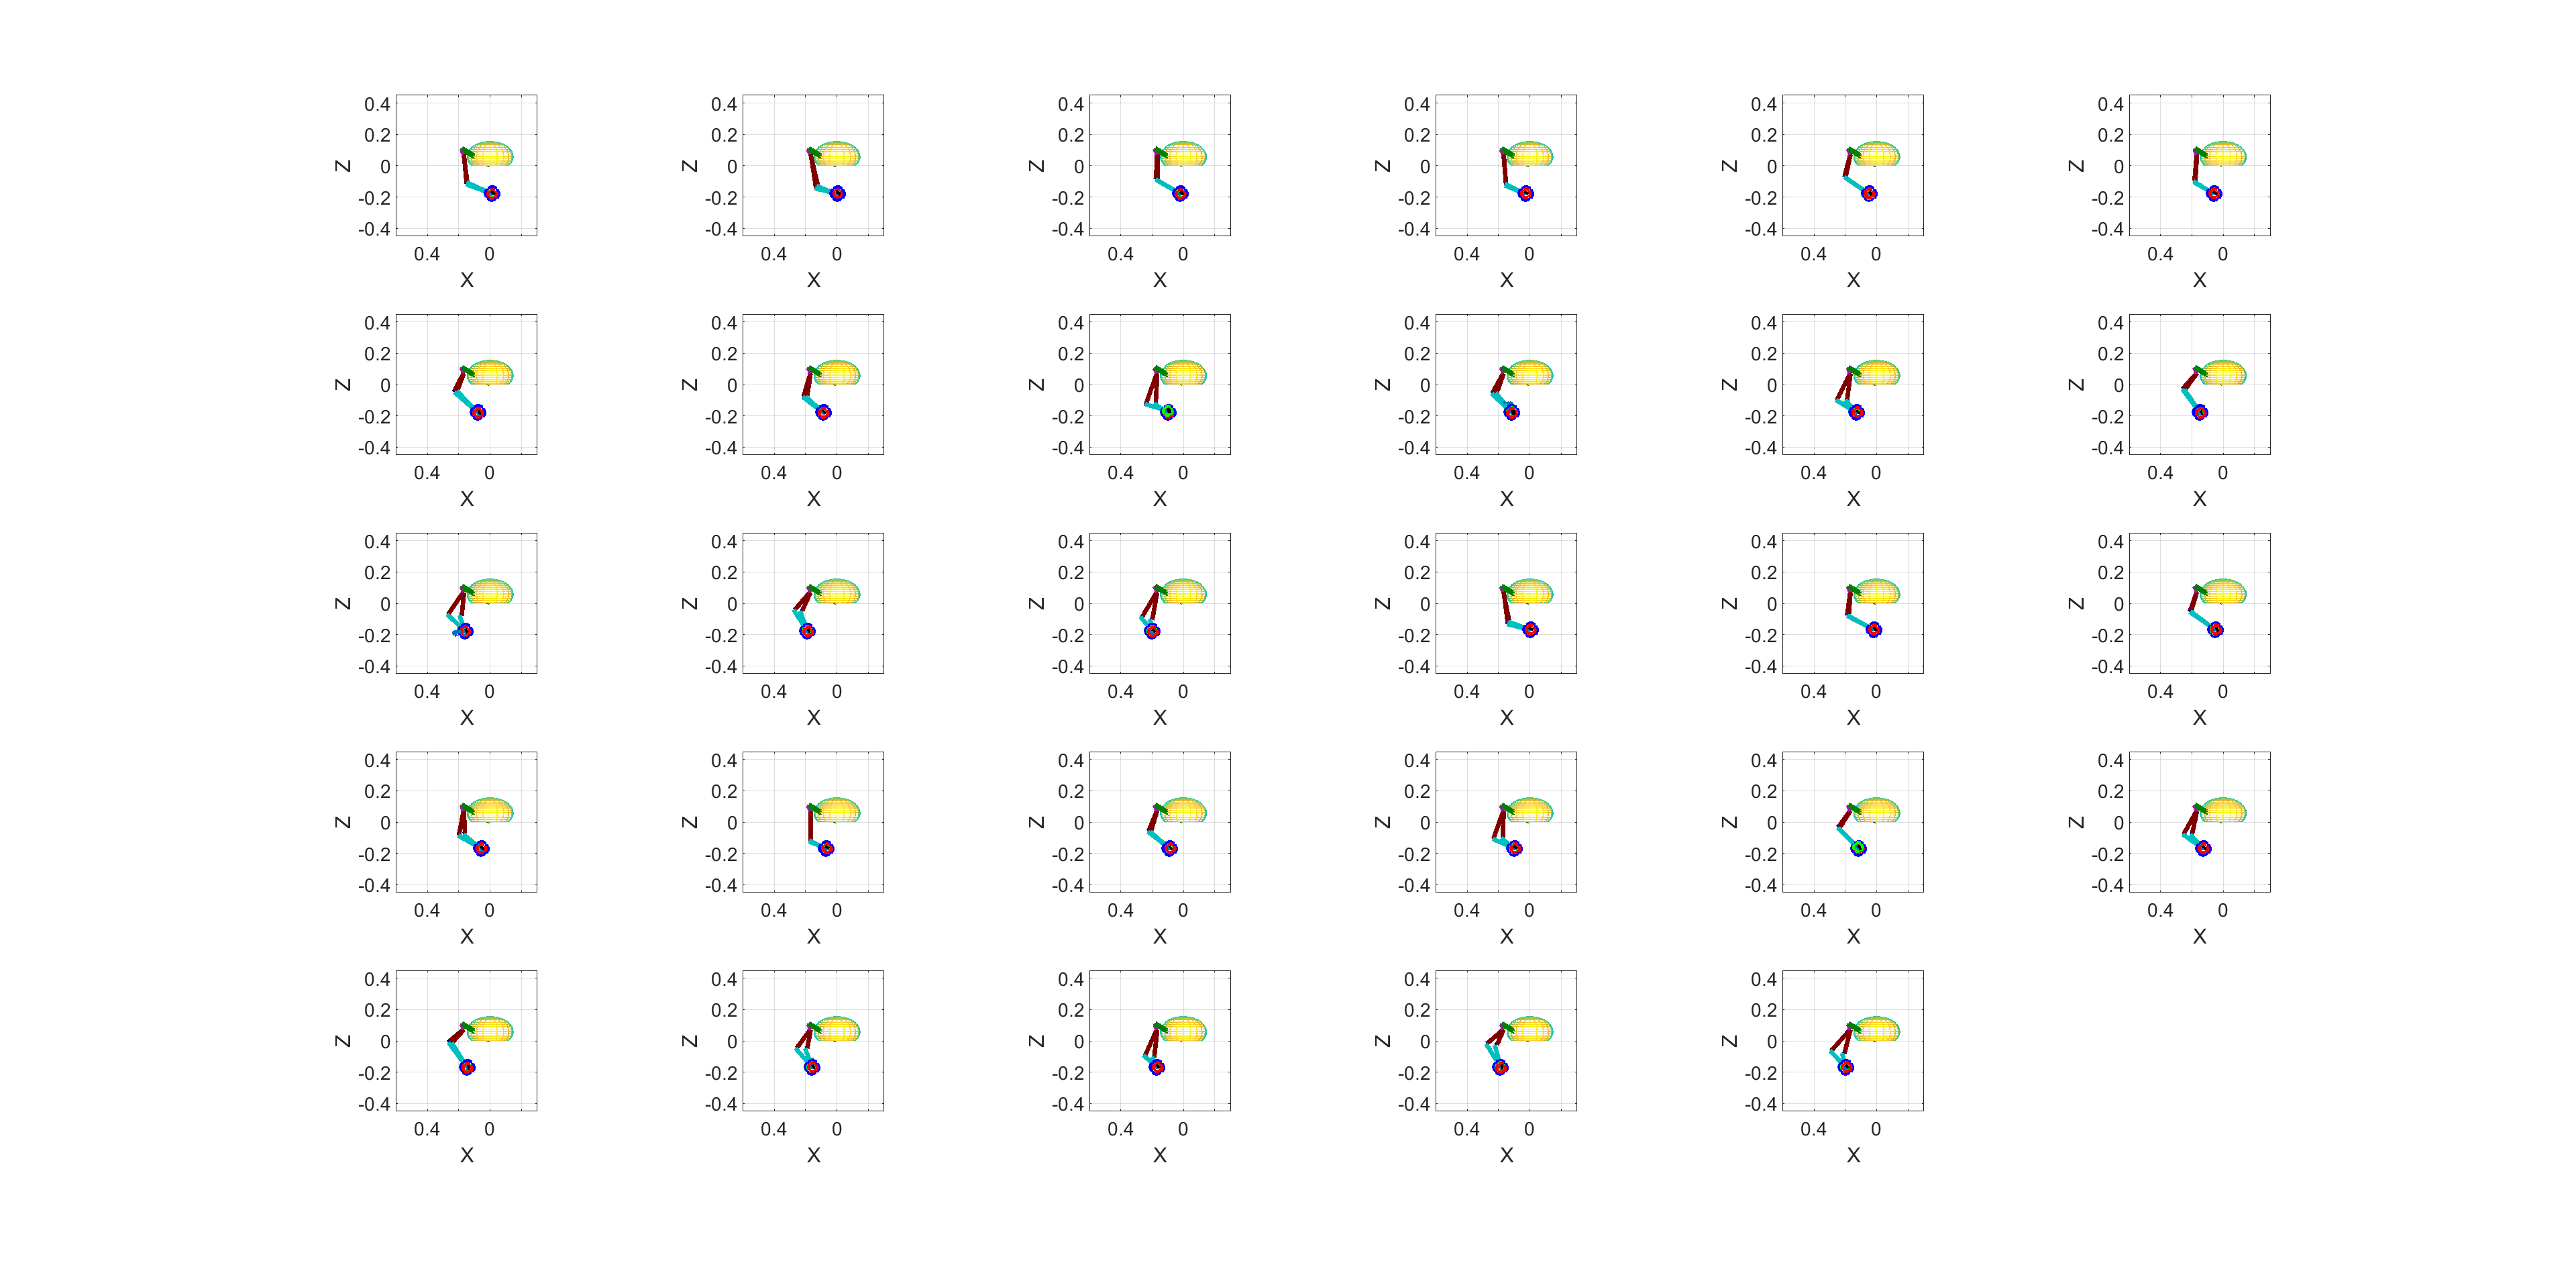
\includegraphics[width=1.9\textwidth]{Pictures/Controller/Static29positions.png} % Replace "filename.jpg" with the name of your image file
    \caption{Desired Targets in Static Control} % Optional caption
  \end{figure}
\end{landscape} % End landscape page




\subsection{Path Following Quasi-Static Control}
\begin{figure}[h!]
\centering
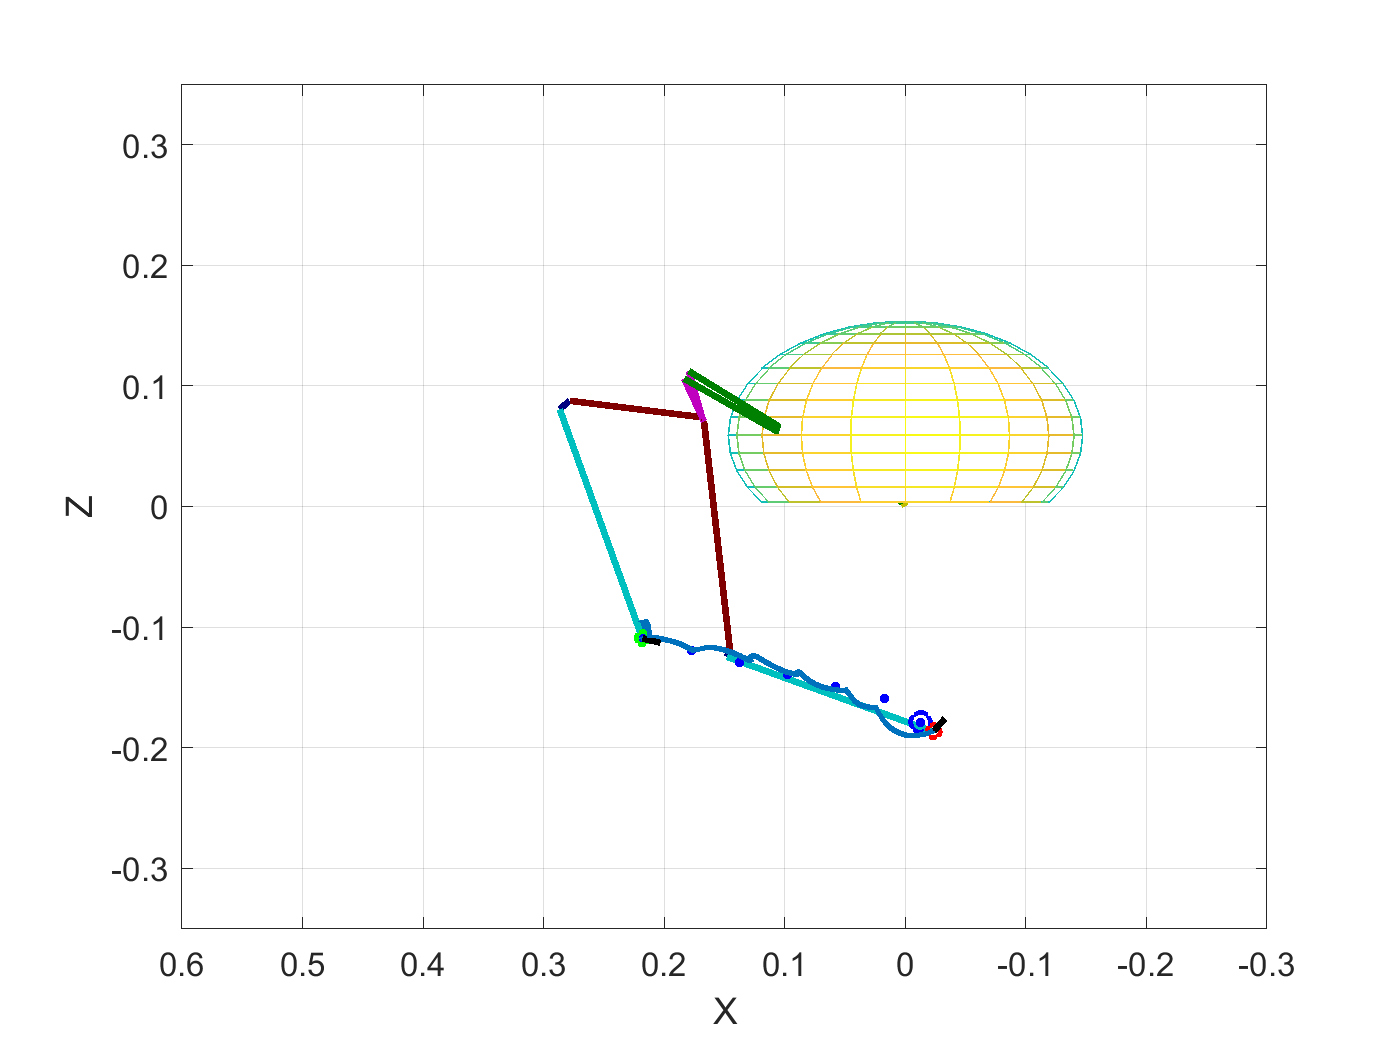
\includegraphics[width=0.75\textwidth]{Pictures/Controller/Healthy_WP.png} 
\caption{Path Following Quasi-Static Control Wrist Position} % Optional caption
\label{fig:PFWP} % Optional label for referencing
\end{figure}

\begin{figure}[h!]
\centering
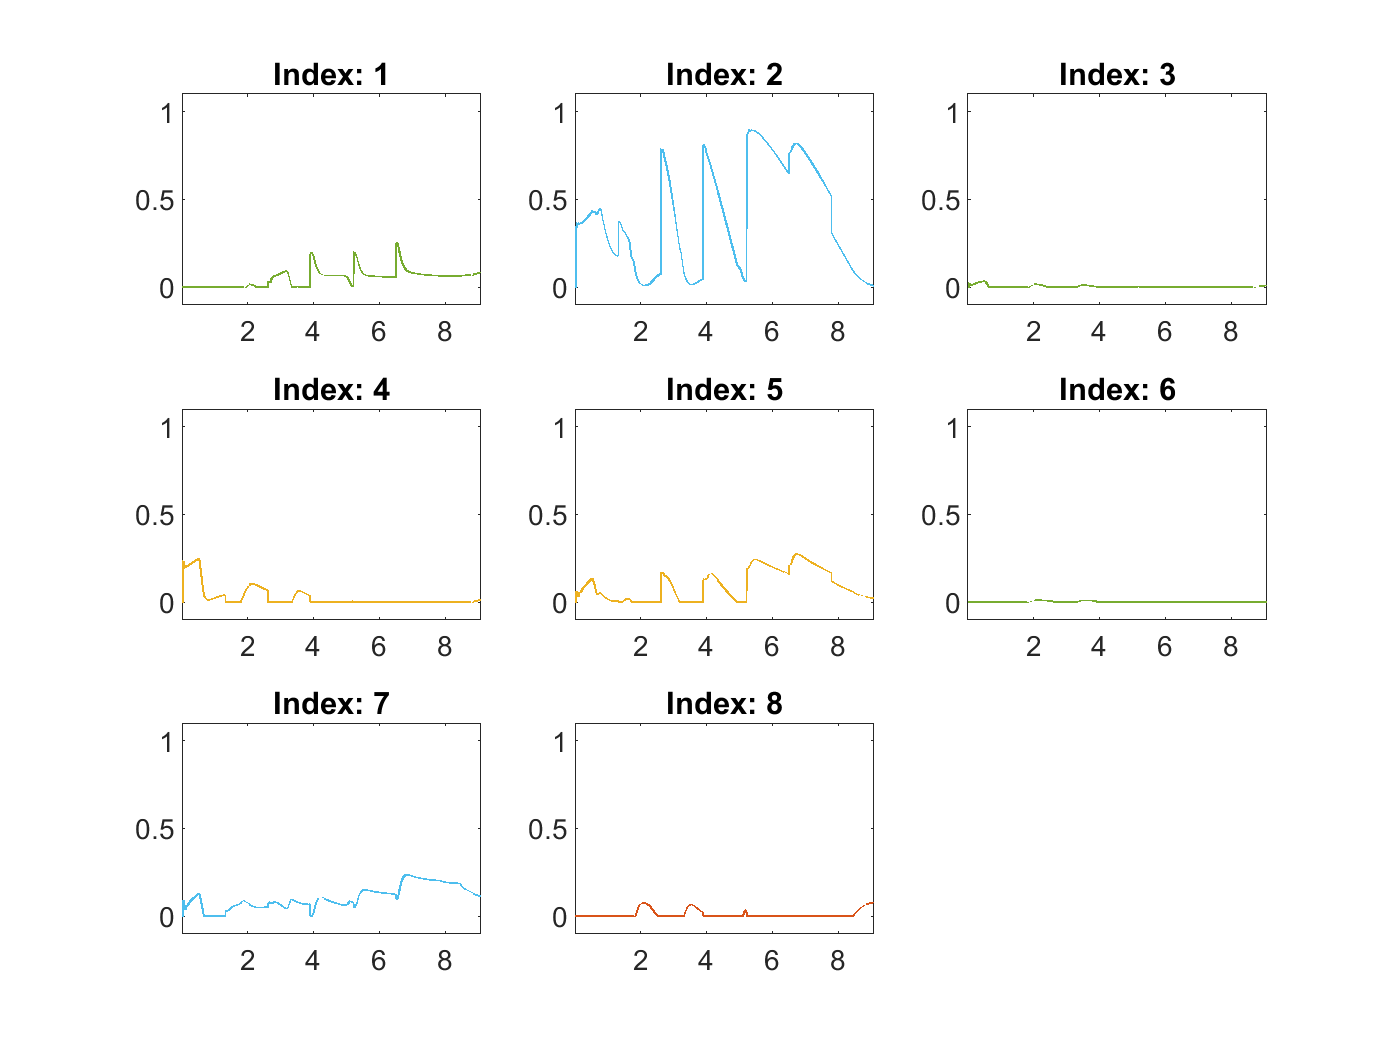
\includegraphics[width=1\textwidth]{Pictures/Controller/Healthy_NA.png} 
\caption{Path Following Quasi-Static Control Neural Activation} % Optional caption
\label{fig:PFNA} % Optional label for referencing
\end{figure}

\newpage
\begin{landscape} % Start landscape page
  \begin{figure}[h!]
    \centering
    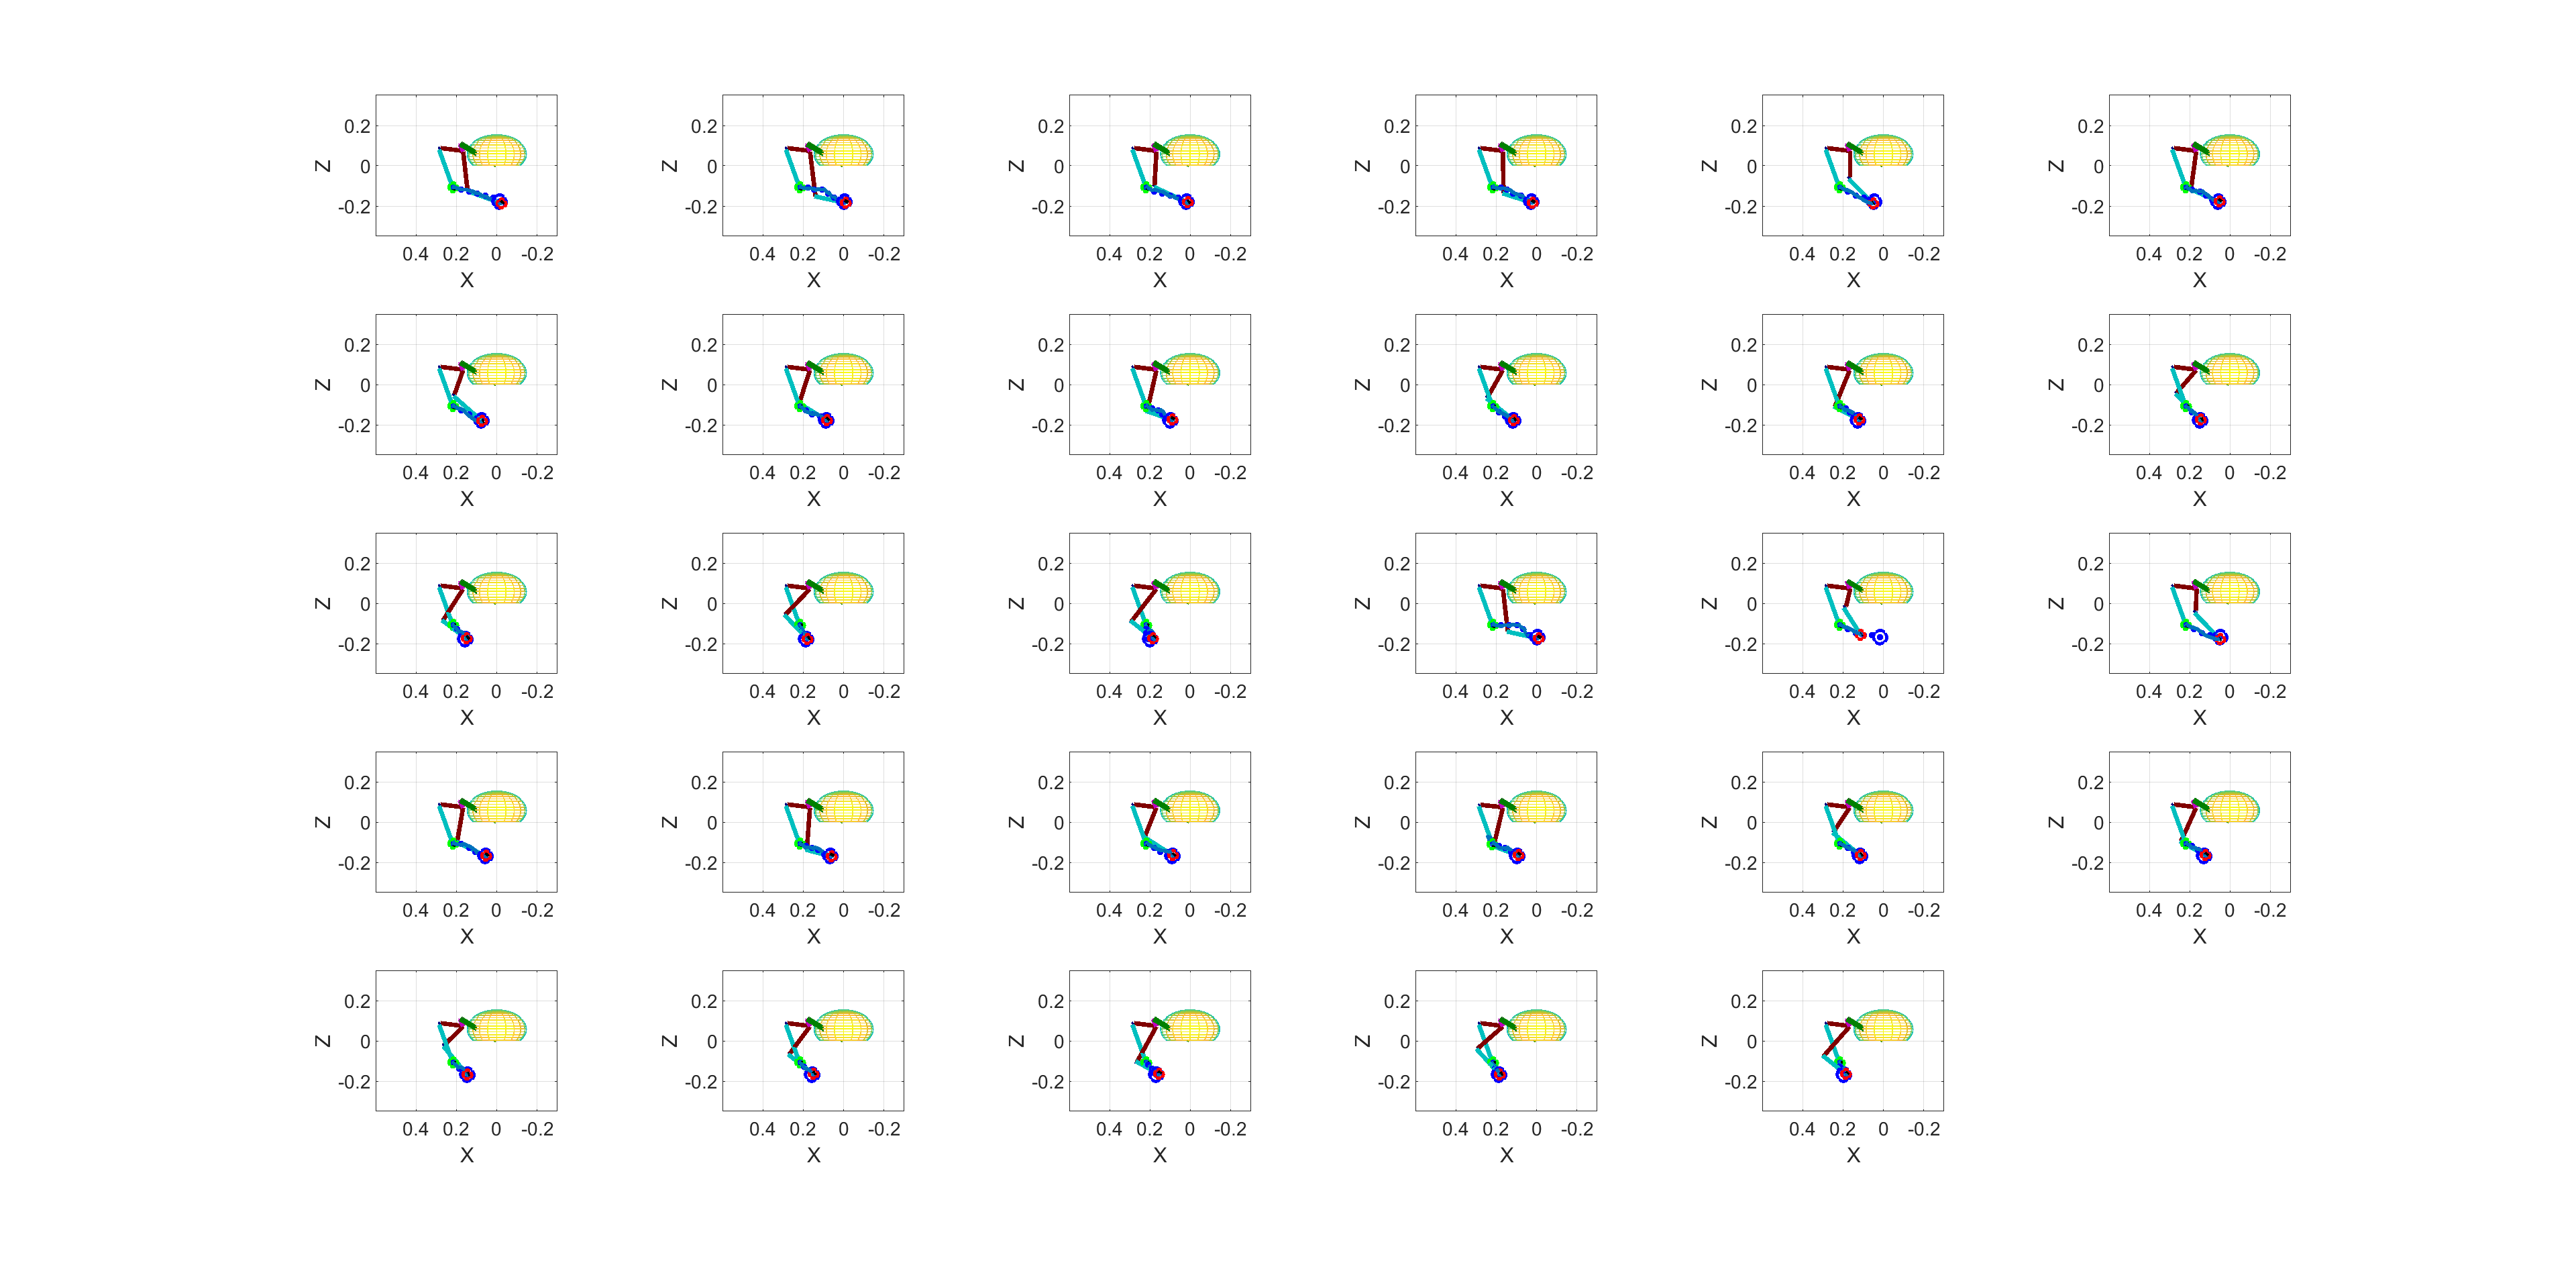
\includegraphics[width=1.7\textwidth]{Pictures/Results/Controller/QSC29positions.png}
    \caption{Desired Targets in Path-Following Quasi-Static Control} 
  \end{figure}
\end{landscape} % End landscape page

\subsection{EMG-Influenced Control}

\begin{figure}[h!]
\centering
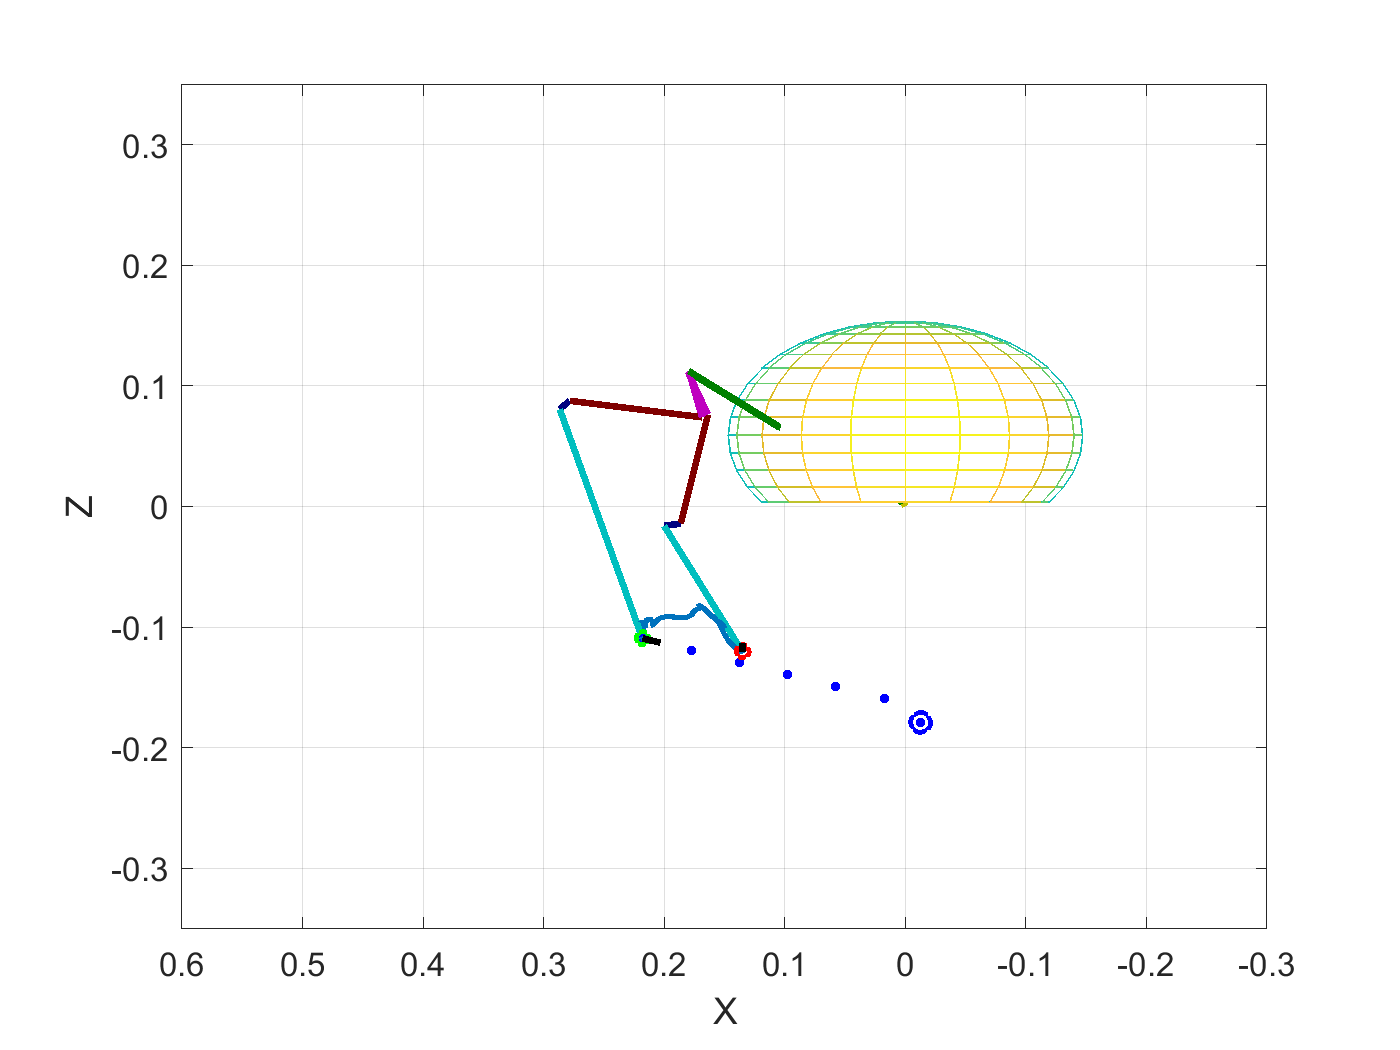
\includegraphics[width=0.75\textwidth]{Pictures/Results/Controller/StrokeWithouControl_WP.png} 
\caption{Stroke = 7 Without EMG-Influence Control Wrist Position} % Optional caption
\label{fig:WOEMGWP} % Optional label for referencing
\end{figure}

\begin{figure}[h!]
\centering
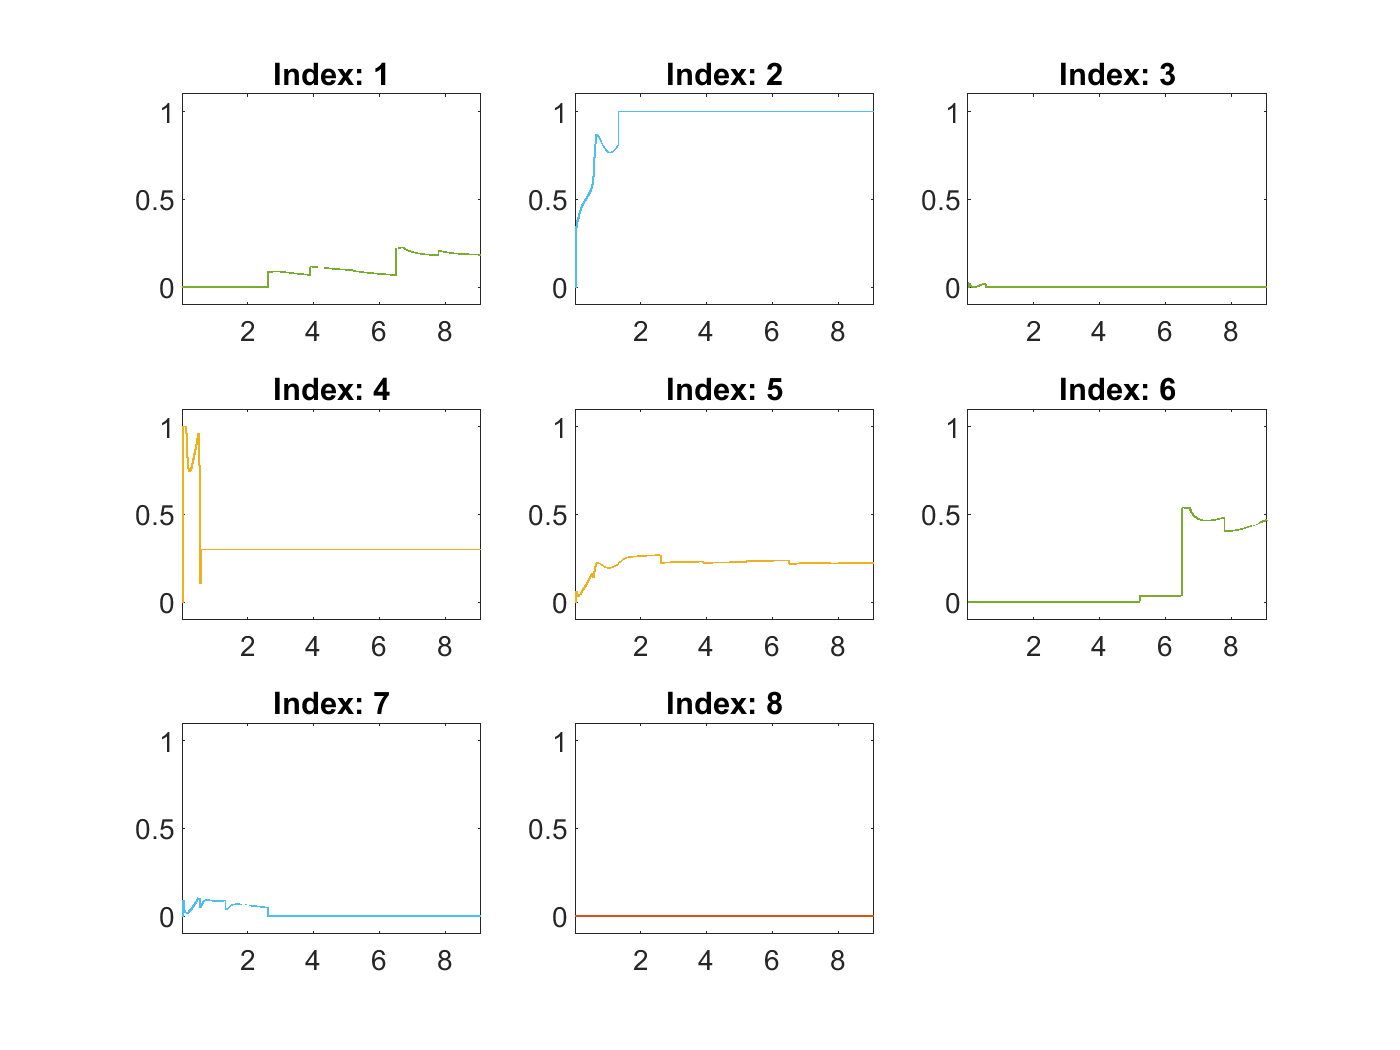
\includegraphics[width=1\textwidth]{Pictures/Results/Controller/StrokeWithouControl_NA.png} 
\caption{Stroke = 7 Without EMG-Influence Control Neural Activation} % Optional caption
\label{fig:WOEMGNA} % Optional label for referencing
\end{figure}


\newpage
\begin{landscape} % Start landscape page
  \begin{figure}[h!]
    \centering
    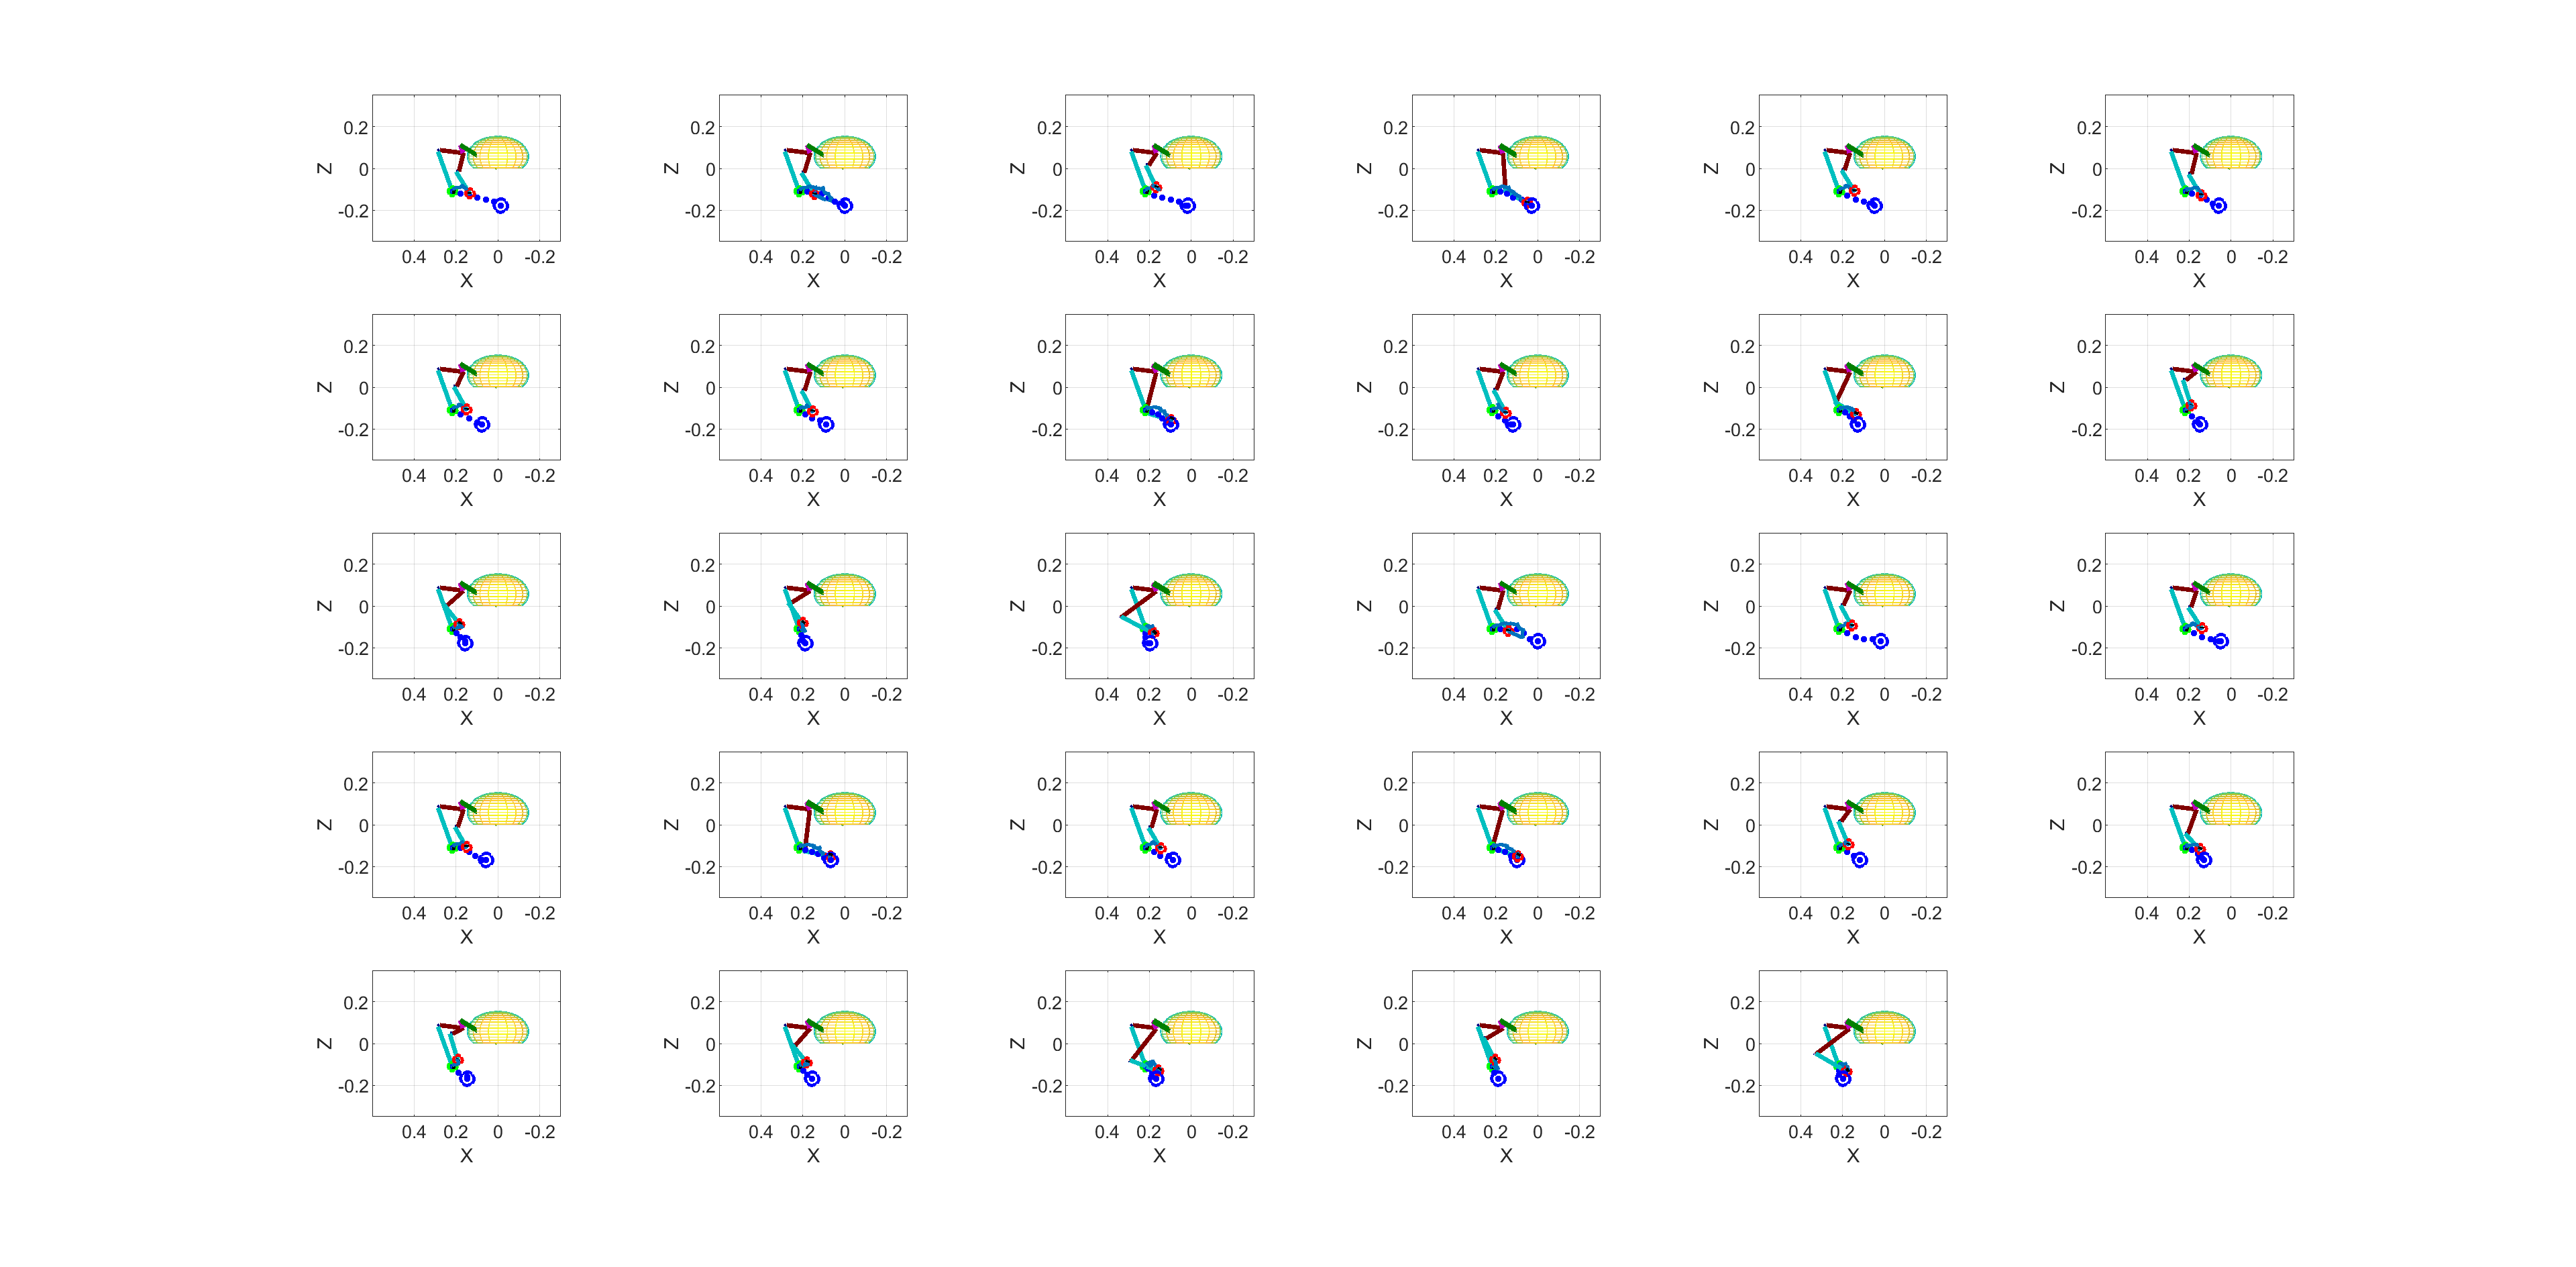
\includegraphics[width=1.9\textwidth]{Pictures/Results/Controller/WithStroke29positions.png} % Replace "filename.jpg" with the name of your image file
    \caption{Desired Targets With Stroke = 7 Without EMG-Influenced Control} % Optional caption
  \end{figure}
\end{landscape} % End landscape page


\begin{figure}[h!]
\centering
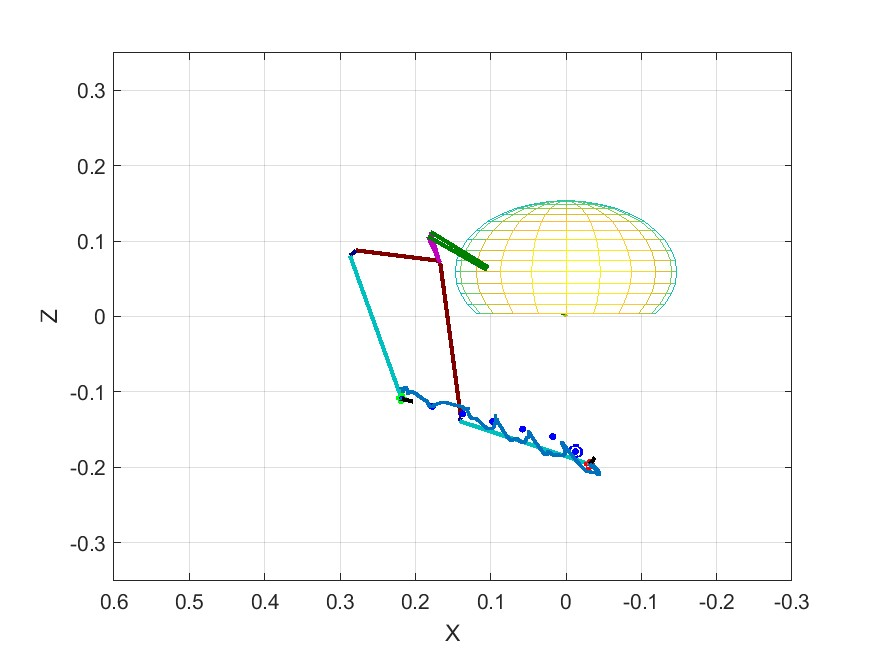
\includegraphics[width=0.75\textwidth]{Pictures/Results/Controller/G(2.99)_G(14.48)_Stroke_7_position_totry(5485)_wp.jpg} 
\caption{Stroke = 7 With EMG-Influence Control Wrist Position} % Optional caption
\label{fig:EMGWP} % Optional label for referencing
\end{figure}

\begin{figure}[h!]
\centering
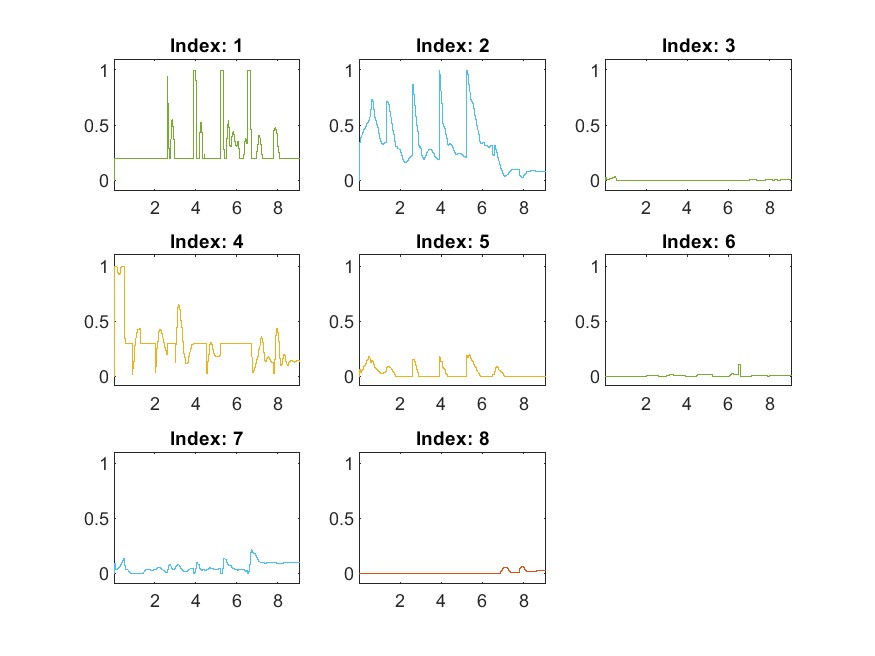
\includegraphics[width=1\textwidth]{Pictures/Results/Controller/G(2.99)_G(14.48)_Stroke_7_position_totry(5485).png_ne.jpg} 
\caption{Stroke = 7 With EMG-Influence Control Neural Activation} % Optional caption
\label{fig:EMGNA} % Optional label for referencing
\end{figure}

\newpage
\begin{landscape} % Start landscape page
  \begin{figure}[h!]
    \centering
    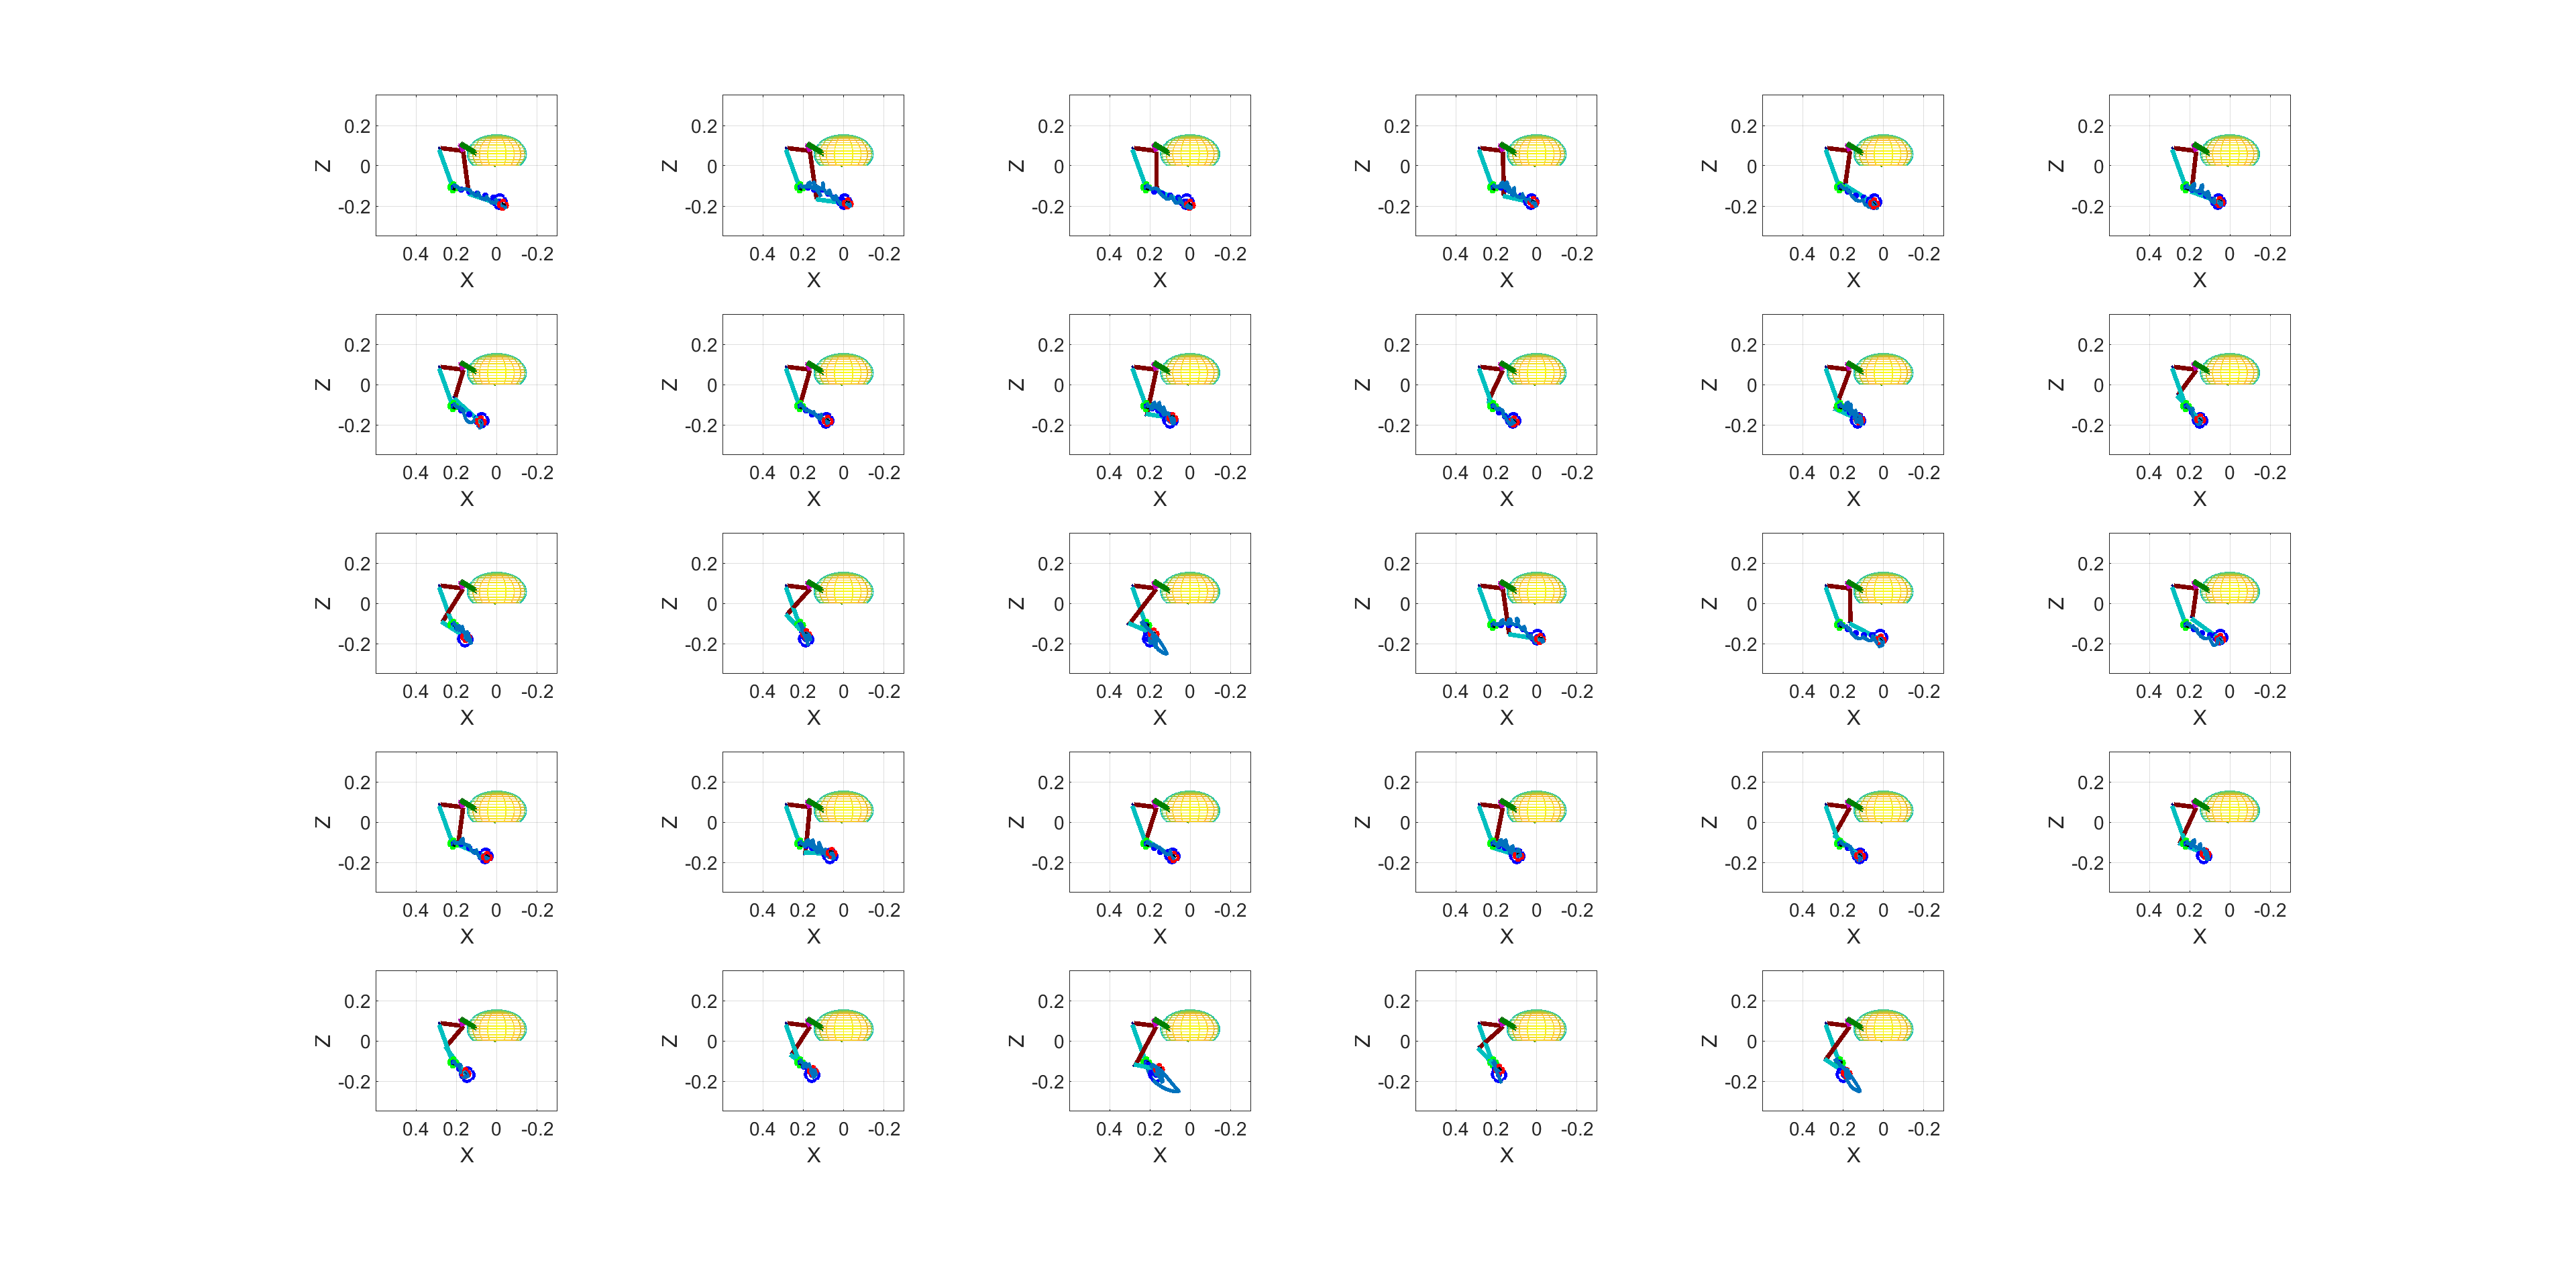
\includegraphics[width=1.9\textwidth]{Pictures/Results/Controller/Stroke29positions.png}
    \caption{Desired Targets With Stroke = 7 With EMG-Influenced Control} 
  \end{figure}
\end{landscape} % End landscape page